\chapter{Introduzione ai S. D.}
Cominciamo ad introdurre i seguenti argomenti:
\begin{itemize}
    \item Definizione di sistema distribuito
    \item Architetture software
    \item Il modello client-server
    \item Proprietà e caratteristiche fondamentali    
\end{itemize}
\section{Alcune definizioni}
\subsection{Definizione 1}
Ci sono diverse definizioni con alcuni aspetti in particolare in comune.
\\Il libro di testo definire un \textit{sistema distribuito} come un sistema in cui componenti hardware o software che sono localizzati in un sistema collegato alla rete, \textbf{comunicano} e \textbf{coordinano} le loro azioni solamente (\textbf{"only by"}) passandosi messaggi.
\\In inglese: "We define a distributed system as one in which \textbf{hardware or software components} located at \textbf{networked computers} \textbf{communicate} and \textbf{coordinate} their actions \textbf{\textit{only by} passing messages}."
\\Ricorda che stiamo parlando di \textbf{processi}, anche se ci sono processi che operano senza una rete ma sono eccezioni.
\begin{center}
    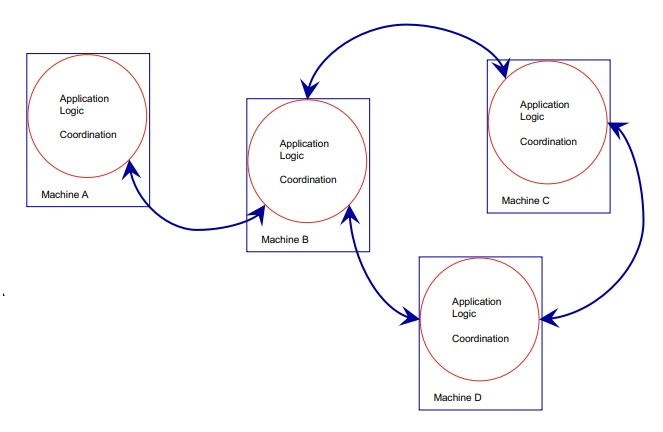
\includegraphics[width=0.75\textwidth]{img/lez28022023_def1.jpg}
\end{center}

\subsection{Definizione 2}
Un'altra definizione è la seguente.
\\Un \textit{sistema distribuito} è definito come un sistema di \textbf{elementi computativi autonomi} (che coesistono) che appaiono ad un utente come un'unica applicazione, un \textbf{unico sistema coerente}.
\\In inglese: "A distributed system is a collection of \textbf{autonomous computing elements} that appears to its users as a \textbf{single coherent system}."
\begin{center}
    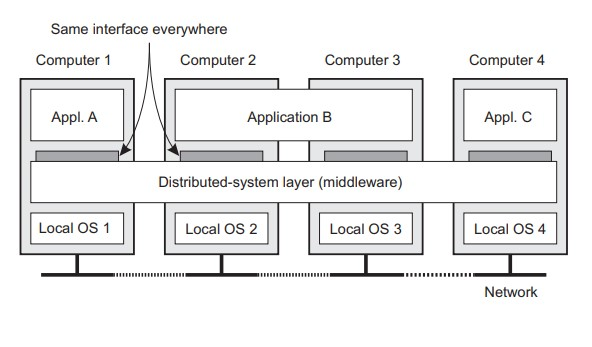
\includegraphics[width=0.75\textwidth]{img/lez28022023_def2.jpg}
\end{center}

\subsection{In sintesi}
Definizione:
\begin{itemize}
    \item Un sistema distribuito è definito come un sistema di elementi computativi autonomi che coesistono e che appaiono ad un utente come un'unica applicazione, un unico sistema coerente.
\end{itemize}
Caratteristiche tipiche:
\begin{itemize}
   \item Elementi computativi autonomi, anche noti come \textit{nodi}; composti da device hardware o processi software
   \item Unico sistema coerente: gli utenti o le applicazioni percepiscono un singolo sistema
\end{itemize}
$\Rightarrow$ i nodi \textbf{devono collaborare}.

\section{Sistemi come collezioni di nodi autonomi}
\subsection{Comportamenti}
Sono \textbf{autonomi} e \textbf{indipendenti}, ovvero possono progredire come vogliono, ognuno ha la propria concezione del tempo $\Rightarrow$ \textit{non} c'è un clock globale, \textit{non} è tutto sincronizzato.
\\Tutto ciò porta a \textit{fondamentali problemi} di \textbf{sincronizzazione} e \textbf{coordinazione}.

\subsection{Collezioni di nodi}
Come gestire \textbf{appartenenze di gruppo} (o \textit{group membership})?
\\I \textbf{gruppi} possono essere \textbf{aperti/dinamici} (qualunque nodo può partecipare) o \textbf{chiusi/fissi} (solo nodi ben selezionati possono entrare nel sistema, questa nozione verrà commentata ulteriormente e comunque non troppo a fondo).
\\Ma quindi, come faccio a sapere se il nodo con cui sto comunicando è effettivamente \textbf{autorizzato}? Non ha proprio risposto.

\section{Sistemi coerenti}
\subsection{Essenzialmente}
La collezione di nodi opera nello stesso modo indipendentemente da dove, quando e come avvengono le interazioni fra l'utente e il sistema.
\\Esempi
\begin{itemize}
    \item Un utente finale (end user) non può dire dove stia avvenendo una computazione
    \item Dove i dati sono collezionati e stipati non dovrebbe essere rilevante per un'applicazione
    \item Se i dati siano stati replicati o meno è completamente nascosto
\end{itemize}

\subsection{Trasparenza di come caratteristica fondamentale dei sistemi distribuiti}
\textbf{"Trasparenza di distribuzione (?)"} come parola chiave. Da tradurre.
Il problema principale: \textbf{fallimenti parziali}.
\begin{itemize}
    \item \`E inevitabile che in qualsiasi momento solo una parte limitata del sistema distribuito fallisca.
    \item Nascondere fallimenti parziali e il loro ripristino è spesso molto complicato e generalmente impossibile da nascondere.
\end{itemize}

\section{Sintesi delle caratteristiche di un sistema distribuito}
Caratteristiche fondamentali per tutti i sistemi distribuiti:
\subsubsection{Gestione della memoria?}
\begin{itemize}
    \item \textbf{Non c'è memoria condivisa}
    \item Comunicazione via scambio messaggi
    \item Non c'è stato globale: ogni componente (nodo, processo) conosce solo il proprio stato e può sondare lo stato degli altri.
\end{itemize}

\subsubsection{Gestione dell'esecuzione?}
\begin{itemize}
    \item \textbf{Ogni componente è autonomo} => esecuzione concorrente
    \item Il coordinamento delle attività è importante per definire il comportamento di un sistema/applicazione costituita da più componenti
\end{itemize}

\subsubsection{Gestione del tempo (temporizzazione)?}
\begin{itemize}
    \item \textbf{Non c'è un clock globale}
    \item Non c'è possibilità di controllo/scheduling globale
    \item Solo coordinamento via scambio messaggi
\end{itemize}

\subsubsection{Tipi di fallimenti?}
\begin{itemize}
    \item \textbf{Fallimenti indipendenti} dei singoli nodi (independent failures)
    \item Non c'è fallimento globale
\end{itemize}

% ----------------------------------------------------------------------------------------------------------------------------------------

\chapter{Architetture Software}
\section{Definizione di architetture software}
Un'architettura software definisce la struttura del sistema, le interfacce tra i componenti e i pattern di interazione (i protocolli). 
\\I sistemi distribuiti possono essere organizzati secondo \textbf{diversi stili architetturali}.

\section{Modello base: Architetture a strati (layered)}
\begin{itemize}
    \item Sistemi operativi
    \item Middleware
\end{itemize}
\subsection{Definizione}
Un'\textit{architettura a strati} è un'architettura software che \textit{organizza il software in \textbf{strati}}.
\\Ogni strato è \textit{costruito sopra uno strato diverso più generico}.
\\Uno strato può essere definito liberamente insieme di (sotto)sistemi con lo \textit{stesso grado di generalità}.
\\\textit{Gli strati più alti sono più specifici per applicazioni e i più bassi sono più generali/generici}.
\begin{center}
    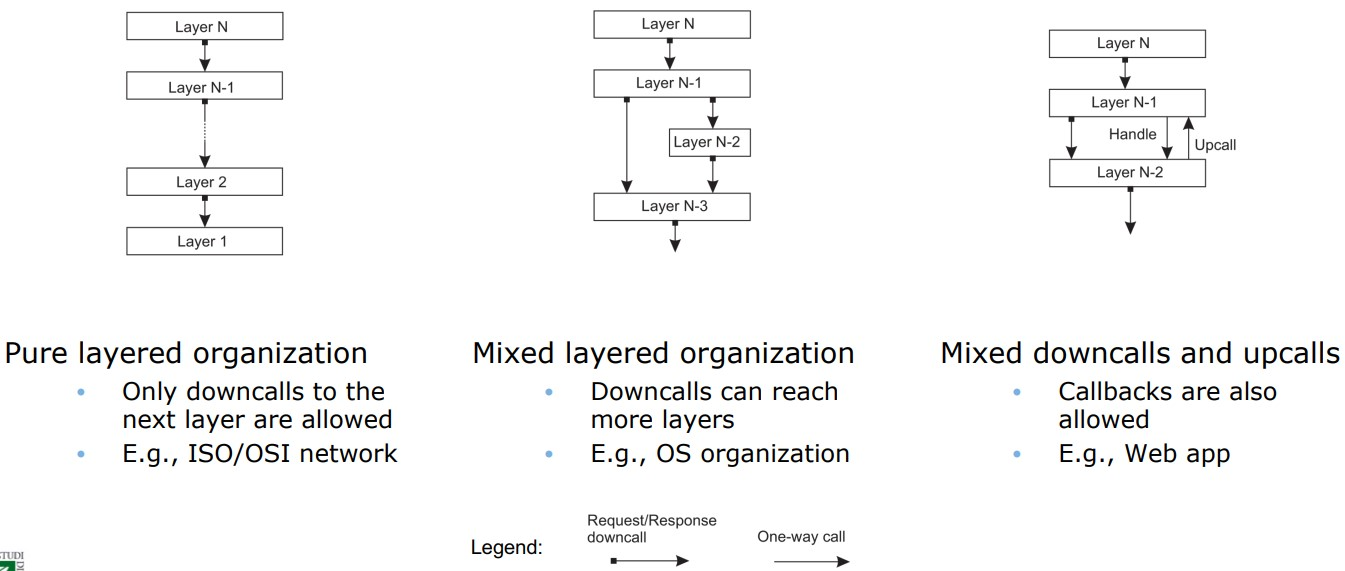
\includegraphics[width=0.5\textwidth]{img/architetturaStrati1.jpg}
\end{center}

\begin{center}
    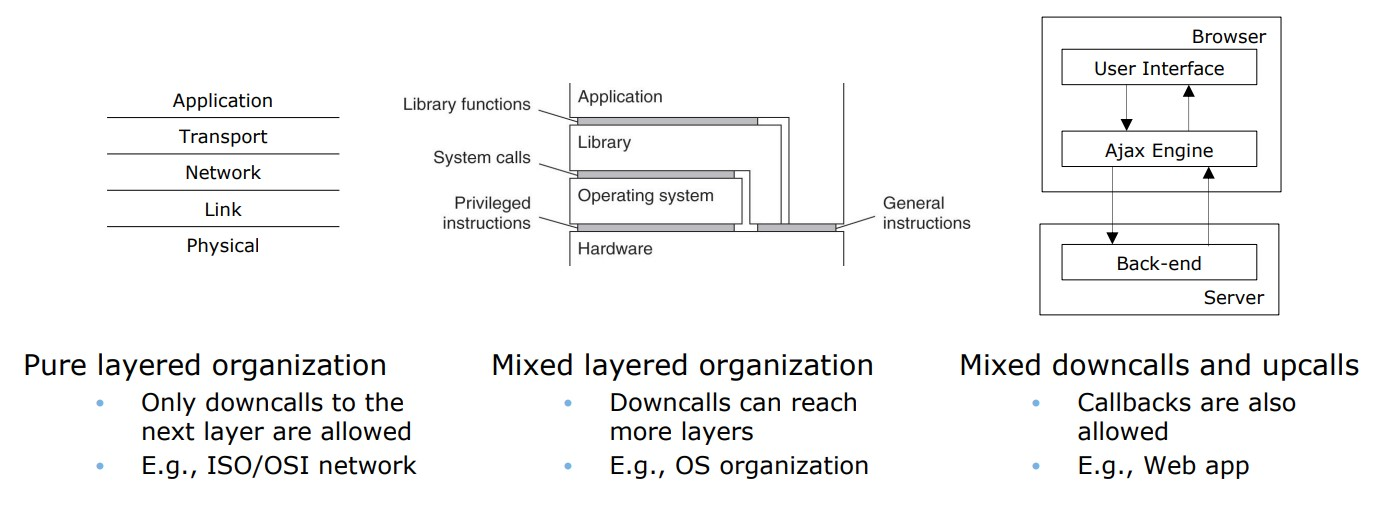
\includegraphics[width=0.5\textwidth]{img/architetturaStrati2.jpg}
\end{center}
Quella al centro è da sapere benissimo in quanto oggetto di questo insegnamento.

%  ------------------------------------------------------

\section{Architetture a livelli (tier)}
\begin{itemize}
    \item Le applicazioni client server (2-tier, 3-tier)
\end{itemize}

\section{Architetture basate sugli oggetti}
\begin{itemize}
    \item Java-Remote Method Invocation (RMI)
\end{itemize}

\section{Architetture centrate sui dati}
\begin{itemize}
    \item Il Web come file system condiviso
\end{itemize}

\section{Architetture basate su eventi}
\begin{itemize}
    \item Applicazioni Web dinamiche basate su callback (AJAX)
\end{itemize}

% ----------------------------------------------------------------------------------------------------------------------------------------

\subsection{Sistemi Operativi Ditribuiti}
Diversi tipi: 
\begin{itemize}
    \item DOS (Distributed Operating Systems)
    \item NOS (Network Operating Systems)
    \item Middleware
\end{itemize}
\begin{center}
    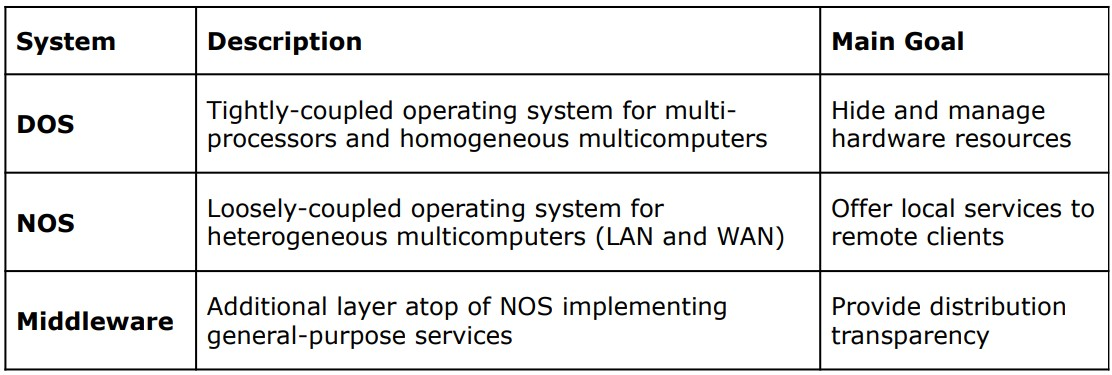
\includegraphics[width=0.5\textwidth]{img/sistemiOperativiDistribuiti1.jpg}
\end{center}

\subsubsection{DOS (Distributed Operating Systems)}
\begin{center}
    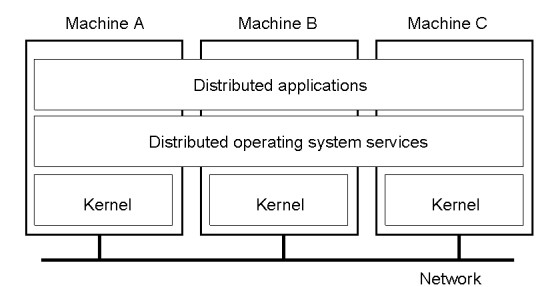
\includegraphics[width=0.5\textwidth]{img/DOS1.jpg}
\end{center}
Users not aware of multiplicity of machines
\begin{itemize}
    \item Access to remote resources like access to local resources
\end{itemize}
Data Migration
\begin{itemize}
    \item Transfer data by transferring entire file, or transferring only those portions of the file necessary for the immediate task
\end{itemize}
Computation Migration
\begin{itemize}
    \item Transfer the computation, rather than the data, across the system
\end{itemize}
Process Migration - execute an entire process, or parts of it, at different sites
\begin{itemize}
    \item Load balancing - distribute processes across network to even the workload
    \item Computation speedup - subprocesses can run concurrently on different sites
    \item Hardware preference - process execution may require specialized processor
    \item Software preference - required software may be available at only a particular site
    \item Data access - run process remotely, rather than transfer all data locally
\end{itemize}

\subsubsection{NOS (Network Operating Systems)}
\begin{center}
    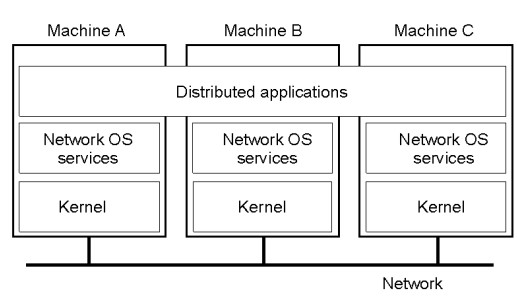
\includegraphics[width=0.5\textwidth]{img/NOS1.jpg}
\end{center}
Users are aware of multiplicity of machines
\\NOS provides explicit communication features
\begin{itemize}
    \item Direct communication between processes (socket)
    \item Concurrent (i.e., independent) execution of processes that from a distributed application
    \item Services, such as process migration, are handled by applications
\end{itemize}
Access to resources of various machines is done explicitly by:
\begin{itemize}
    \item Remote logging into the appropriate remote machine (telnet, ssh)
    \item Remote Desktop (Microsoft Windows)   
    \item Transferring data from remote machines to local machines, via the File Transfer Protocol (FTP) mechanism
\end{itemize}

\subsubsection{Middleware}
\begin{center}
    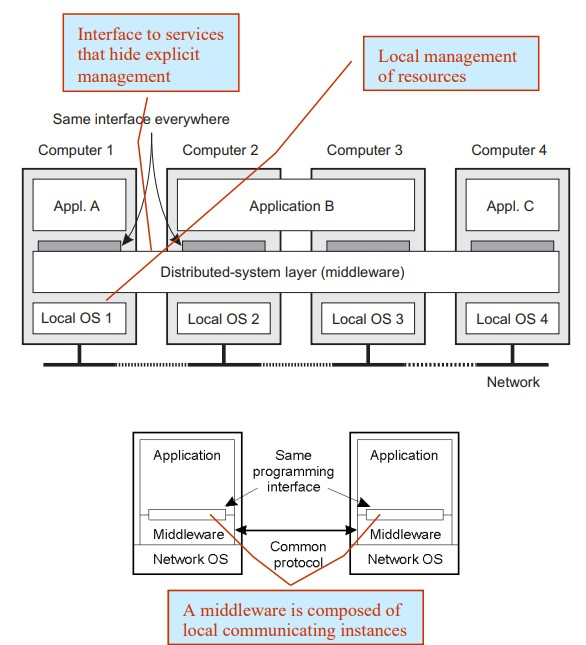
\includegraphics[width=0.5\textwidth]{img/Middleware1.jpg}
\end{center}
Distributed Operating Systems
\begin{itemize}
    \item Make services (e.g., data storage and process execution) \textbf{transparent} to applications
    \item Rely on homogeneous machines (since they need to run the same software)
\end{itemize}
Network Operating Systems
\begin{itemize}
    \item Services (e.g., data storage and process execution) \textbf{are explicitly managed} by applications
    \item Do not require homogeneous machines (since they may run different software)
    \item E.g., MacOSX, Windows10, Linux
\end{itemize}
Middleware
\begin{itemize}
    \item Implements services (one or more) to \textbf{make them transparent} to applications
    \item E.g., Java/RMI
\end{itemize}
è importante capire che nel secondo schema dell'immagine, il middleware simula il comportamento dell'applicazione, ma i due middleware sono uguali ma possono comunicare tramite protocolli.

\subsubsection{Servizi Middleware}
Services can address several issues, from general to domain specific.
\\Naming (il più importante) ovvero come faccio ad identificare un sistema operativo: astrazione
\begin{itemize}
    \item Symbolic names are used to identify entities that are part of a DS
    \item They can be used by registries to provide the real addresses (e.g., DNS, RMI registries), or implicitly by the middleware
\end{itemize}
Access transparency (il più importante)
\begin{itemize}
    \item … defines and offers a communication model that hides details on message passing
\end{itemize}
Persistence
\begin{itemize}
    \item … defines and offers an automatic service for data storage (on file system or DB)
\end{itemize}
Distributed transactions (non vedremo tanto a fondo)
\begin{itemize}
    \item … defines and offers a persistence models to automatically ensure consistency on read/write operations (usually on DBs)
\end{itemize}
Security (non vedremo tanto a fondo)
\begin{itemize}
    \item … defines and offers models to protect access to data and services (with different levels of permissions) and computation integrity
\end{itemize}
\begin{center}
    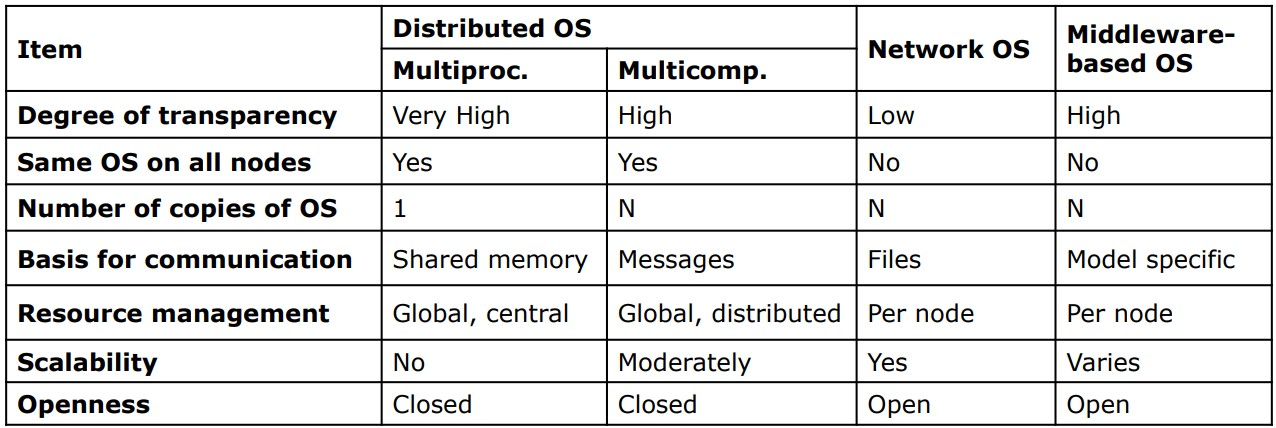
\includegraphics[width=0.5\textwidth]{img/confrontoFraSistemi1.jpg}
\end{center}

% ----------------------------------------------------------------------------------------------------------------------------------------

\chapter{Il modello Client-Server}
Il modello Client-Server è il modello di interazione tra un processo client e un processo server.
\begin{center}
    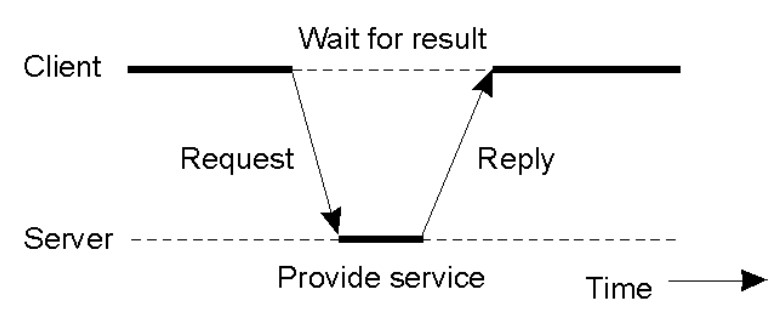
\includegraphics[width=0.5\textwidth]{img/modelloCS1.jpg}
\end{center}